\documentclass[12pt]{article}

\usepackage{graphicx}
\usepackage[utf8]{inputenc}
\usepackage[english,russian]{babel}
\usepackage[pdftex,unicode]{hyperref}
\usepackage[margin=15mm,left=2cm]{geometry}
\usepackage{indentfirst}
\usepackage{amsbib}
\usepackage{amsmath}

\sloppy
\clubpenalty=999
\widowpenalty=9999

\newtheorem{theorem}{Теорема}[section]
\newtheorem{lemma}[theorem]{Лемма}
\newtheorem{proposition}[theorem]{Утверждение}
\newtheorem{corollary}[theorem]{Следствие}

\newenvironment{proof}[1][Доказательство]{\begin{trivlist}
\item[\hskip \labelsep {\bfseries #1}]}{\end{trivlist}}
\newenvironment{definition}[1][Определение]{\begin{trivlist}
\item[\hskip \labelsep {\bfseries #1}]}{\end{trivlist}}
\newenvironment{example}[1][Example]{\begin{trivlist}
\item[\hskip \labelsep {\bfseries #1}]}{\end{trivlist}}
\newenvironment{remark}[1][Замечание]{\begin{trivlist}
\item[\hskip \labelsep {\bfseries #1}]}{\end{trivlist}}

\newcommand{\qed}{\nobreak \ifvmode \relax \else
      \ifdim\lastskip<1.5em \hskip-\lastskip
            \hskip1.5em plus0em minus0.5em \fi \nobreak
                  \vrule height0.75em width0.5em depth0.25em\fi}

% This is all for formatting and making the Table of Contents according to 
% spec. Don't play with it.
\makeatletter
\renewcommand\l@section[2]{%
    \ifnum \c@tocdepth >\z@
        \addpenalty\@secpenalty
        \addvspace{1.0em \@plus\p@}%
        \setlength\@tempdima{1.5em}%
        \begingroup
        \parindent \z@ \rightskip \@pnumwidth
        \parfillskip -\@pnumwidth
        \leavevmode \bfseries
        \advance\leftskip\@tempdima
        \hskip -\leftskip
#1\nobreak\ 
        \leaders\hbox{$\m@th\mkern \@dotsep mu\hbox{.}\mkern \@dotsep mu$}
    \hfil \nobreak\hb@xt@\@pnumwidth{\hss #2}\par
        \endgroup
    \fi}
\makeatother

\title{Критерий для класса предикатных схем}
\author{Василевская И.\,Ю.}
\date{\today}

\begin{document}
    \begin{titlepage}
        \begin{center}
            Московский Государственный Университет им. Ломоносова\\
            Факультет Вычислительной Математики и Кибернетики\\
            Кафедра Математической Кибернетики\\
            магистратура, отделение <<МММ СБИС>>\\[6cm]

            \large {Василевская Инесса Юрьевна}\\
            \LARGE \textbf {Верхние оценки одного параметра для класса предикатных схем}\\[0.8cm]
            \large \emph {Курсовая работа}\\[5.0cm]

            \begin{flushright}
                \large
                \begin{minipage}{0.40\textwidth}
                    \begin{flushleft}
                        \emph{Научный руководитель:}\\к.ф.м.н М.\,С.~Шуплецов
                    \end{flushleft}
                \end{minipage}
            \end{flushright}

            \vfill
            Москва\\
			2012
        \end{center}
    \end{titlepage}

\setcounter{page}{2}

\section{Введение}
\label{beginning}
В ряде работ (\cite{Shu09}, \cite{Shu11}) рассматривается задача синтеза для специального класса дискретных управляющих систем ~--
класса предикатных схем, который обобщает некоторые традиционные классы схем. Данные схемы строятся из предикатных элементов
и обладают рядом отличий от схем из других классов (например, направление протекания сигналов не является фиксированным).
Указанные выше работы в основном посвящены исследованию асимптотики функции Шеннона в классе предикатных схем,
 получению асимптотических оценок высокой степени точности и вопросам моделирования предикатными схемами схем из традиционных классов.

В силу особенностей класса предикатных схем, при его рассмотрении могут возникать вопросы,
нетипичные для традиционных классов. Так, к примеру, довольно любопытен вопрос функционирования предикатных схем с точки зрения оценки времени, которое нужно затратить для
вычисления конкретной схемы. 
В данной работе в качестве меры <<быстрой вычислимости>>\footnote{в англоязычной литературе употребляется термин tracktability}
 был выбран так называемый параметр \textit{ширины декомпозиции}~-- максимального числа вершин в узле дерева, 
которое можно оптимально построить по заданной предикатной схеме. Во многих работах (например, \cite{CSP10}, \cite{Gott10}, \cite{Prosc89}) было 
показано, что задачи, которые можно переформулировать в терминах Constraint Satisfaction Problem, быстро вычислимы, если ширина декомпозиции графа ограничений 
(constraint graph) ограничена сверху константой. 
Так как задача функционирования предикатных схем естественным образом представляется как задача CSP с булевыми ограничениями,
 вопрос <<быстрой вычислимости>> заданного предиката в конкретном базисе сводится к нахождению такого способа синтеза, 
 при котором результирующая схема будут иметь ограниченный параметр ширины декомпозиции
\footnote
{В англоязычных источниках известного как treewidth. В силу отсутствия общепринятого перевода, автор вводит 
понятие ``ширины декомпозиции''}.

\clearpage
\section{Основные определения}
Ниже приведены формальные определения используемых в работе понятий.

\subsection{Предикатные схемы}

В настоящей работе определение предикатных схем будет дано по аналогии с \cite{Shu11}.

\begin{definition}
\textit{Схемой из предикатных элементов} или \textit{предикатной схемой в базисе $\Pi$} назовем помеченный
неориентированный двудольный граф следующей структуры:

\begin{itemize}
\item каждая вершина из первой доли помечена некоторым множеством символов из алфавита X и/или 
множеством символов из алфавита Y. 
Алфавит $X$ соответствует \textit{входным} переменным предиката, а $Y$ ~-- его внутренним переменным, 
т.е. переменным, возникающим непосредственно в процессе вычисления; 

\item каждая вершина второй доли помечена некоторым символом $\pi_i$ из множества $\Pi$ и 
соединена $k$ ребрами, пронумерованными числами $1, ..., k$, с вершинами из первой доли.
\end{itemize}
\end{definition}

Вершины из первой доли будем называть \textit{узлами} схемы, а вершины из второй доли ~-- её \textit{предикатными элементами}. 
Узлы схемы, соединенные ребрами с предикатным элементом, будем называть полюсами этого элемента, 
а узлы, соответствующие входным переменным, ~-- полюсами схемы.
При этом считается, что узел является $j$-м полюсом предикатного элемента и соответствует 
его $j$-ой переменной, если соединяющее их ребро имеет номер $j$. Полюс схемы, которому приписано 
более одной входной переменной, называется кратным полюсом этой схемы. 

Будем считать элементарной такую предикатную схему, которая состоит либо из изолированной полюсной вершины, 
либо только из одного предикатного элемента $\pi_i$, $1 < i < k$, где $k$ ~-- число полюсов указанного элемента.

В тех случаях, когда это не вызывает разночтений, 
не будем различать узел схемы и переменную, 
символ которой приписан данной вершине, а также предикатный элемент и сам предикат, отвечающий этому элементу. 
Также, для удобства, в некоторых случаях будем использовать упрощенное описание предикатной схемы, 
опуская пометки дуг и некоторых внутренних вершин. 

\subsection{Функционирование предикатных схем}
Функционирование предикатного элемента с $k$ полюсами задается его характеристической функцией от $k$ переменных, 
связанных с указанными полюсами, и определяется тем, что предикатный элемент находится в допустимом состоянии на тех и 
только тех наборах значений этих переменных, на которых данная функция равна 1. 

Предикатная схема $\Sigma$ находится в допустимом состоянии на заданном наборе значений её полюсных переменных тогда и только тогда, 
когда существует такой набор значений внутренних переменных схемы, на котором все предикатные элементы схемы находятся в допустимых состояниях. 
Если же указанного набора значений внутренних переменных не существует, то считается, что схема находится в недопустимом состоянии на 
заданном наборе значений её полюсных переменных.

Предполагается, что предикатная схема $\Sigma$ реализует предикат $\pi$ от её полюсных переменных, если множество допустимых наборов $\pi$ 
совпадает с множеством тех наборов, на которых $\Sigma$ находится в допустимом состоянии. 
При этом схемы будем называть эквивалентными, если они реализуют равные предикаты. 
Отметим, что элементарная предикатная схема, состоящая из изолированной полюсной вершины, реализует тождественно истинный предикат.
 Будем считать также, что тождественно истинный (соответственно тождественно ложный)
 предикат реализуется любой предикатной схемой без входных полюсов, 
которая имеет непустое (соответственно пустое) множество допустимых состояний.

В общем случае граф предикатной схемы может содержать несколько компонент связности. 
В дальнейшем, будем считать, что схема не содержит компонент связности, 
которые не имеют полюсных узлов и для которых существует хотя бы один допустимый набор, так как такие компоненты не влияют на функционирование схемы.

\subsection{Операции над предикатными элементами}

Обозначим $\pi(x_1, \dots, x_n)$~-- сам предикат, 
$\Pi(x_1, \dots, x_n)$ ~-- множество его кортежей (наборов значений).

\begin{definition}
Суперпозицией двух предикатных схем, не имеющих общих вершин и пометок, 
будем называть их объединение с возможным отождествлением группы полюсов этих схем, 
которое сопровождается приписыванием новой (``объединенной'') вершине либо 
некоторого подмножества переменных данной группы, либо ``новой'' внутренней переменной.

При этом частными случаями суперпозиции являются следующие операции:

\begin{itemize}
    \item Суперпозиция без отождествления полюсов, или декартово произведение

    В статье \cite{Marchenkov} эта операция соответсвует операции конъюнкции.
    Конъюнкцией $\pi_1(x_1, \dots, x_m)$ и $\pi_2(x_1, \dots, x_n)$ называется такой $(m+n)$-местный предикат $\pi$, что
    $\pi(x_1, \dots, x_m, x_{m+1}, \dots, x_{m+n}) = \pi_1(x_1, \dots, x_m) \& \pi_2(x_{m+1}, \dots, x_{m+n})$.
    Причем множество кортежей $\Pi$ результирующего предиката $\pi$ равно $\Pi_1 \otimes \Pi_2$.

    \item Проекция или снятие полюсной переменной схемы

    По аналогии с \cite{Marchenkov}, проекцией предиката $\pi_1(x_1, \dots, x_n)$ по переменной $x_i$ называется такой
    $(n-1)$-местный предикат $\pi$, что:
    $\pi(x_1, \dots, x_{i-1}, x_{i+1}, \dots, x_n) = (\exists x_i) \pi_1(x_1, \dots, x_{i-1}, x_i, x_{i+1}, \dots, x_n)$.

    \item Суперпозиция с отождествлением полюсов

    Суперпозицией $\pi_1(x_1, \dots, x_m)$ и $\pi_2(y_1, \dots, y_n)$ с отождествлением по первым k переменным 
    называется $(m+n)$-местный предикат
    $\pi(x_1, \dots, x_k, x_{k+1}, \dots, x_m, y_{m+1}, \dots, y_n) = \pi_1(x_1, \dots, x_k, x_{k+1} \dots, x_m) \& \pi_2(x_1, \dots, x_k, y_{k+1}, \dots, y_n)$.

    Сокращенно операцию суперпозиции предикатов $\pi_1$ и $\pi_2$ с отождествлением полюсов 
    $x_1, \dots, x_k$ и $y_1, \dots, y_k$ соответственно, будем обозначать $(\pi_1|\pi_2)_{x_1=y_1, \dots, x_k=y_k}$.

    \item Отождествление двух полюсных переменных схемы

    $\pi(x_1, \dots, x_n) = \pi_1(x_1, x_1, \dots, x_n)$

    \item Подстановка констант $(\sigma_1, \dots, \sigma_k)$ вместо первых k переменных

    $\pi(x_1, \dots, x_n) = \pi_1(\sigma_1, \dots, \sigma_k, x_{k+1}, \dots, x_n)$. 
    Сокращенно операцию подстановки констант вместо переменных $x_1, \dots, x_k$ предиката $\pi$
    будем обозначать $(\pi)|_{x_1=\sigma_1, \dots, x_k=\sigma_k}$.

\end{itemize}
\end{definition}
\section{Сведение модели к обобщенной задаче выполнимости}

\subsection{Обобщенная задача выполнимости}

Формально, \textit{обобщенная задача выполнимости (CSP)}\footnote{Constraint Satisfaction Problem} 
~--- это тройка $<V,D,C>$, где $V$ ~-- набор переменных, $D$ ~-- область определения (домен допустимых значений), 
а $C$ ~-- набор ограничений. Ограничения имеют вид $<t, R_n>$, где $t$ ~--- кортеж из $n$ переменных множества $V$, 
$R_n$ ~-- заданное на $D$ отношение арности $n$. 
Решением задачи CSP является набор значений переменных $V$, который удовлетворяет всем ограничениям из $C$. 

Так, например, задачу 3-ВЫП можно рассматривать как обобщенную задачу выполнимости над булевым доменом, с 
состоящим лишь из отношений-конъюнкций множеством ограничений.

В ряде работ рассматривалась вычислительная сложность задачи CSP. Несмотря на то, что в общем случае задача CSP
принадлежит классу NP, при введении определенных ограничений на множество $C$ или структуру так называемого
графа ограничений\footnote{constraints graph}, существуют быстрые алгоритмы нахождения решения. 
Так, например, в \cite{Shaeffer78} показано, 
что, в тех случаях, когда множество $C$ представляет собой дерево, существуют полиномиальные алгоритмы нахождения решения.

\subsection{Сведение задачи вычисления предикатной схемы к задаче нахождения решения задачи CSP}

Пусть предикатная схема $\Sigma$ имеет $m$ входных переменных $x_1, \ldots , x_m$, 
$k$ внутренних переменных $y_1, \ldots , y_k$ и $n$ предикатных элементов $B = \pi_1, \dots , \pi_n$. 
Тогда, для определения функционирования этой схемы нужно найти допустимые значения внутренних переменных на всех $2^{m}$
наборах входных переменных. 

Нетрудно видеть, что эта задача может быть сведена к $2^m$ задачам CSP $<V, D, C>$ следующим образом:
$V$ = $X \bigcup Y$, $D = [0, 1]$, $C = B$. Перед началом вычисления каждой из задач, переменные $x_1, \ldots , x_m$ 
во всех ограничениях, их содержащих, отождествляются с соответствующими константами $\alpha_1, \ldots , \alpha_m$.

В обеих моделях, сложность вычислений в худшем случае, при применении алгоритма поиска 
с откатом без памяти, требует $2^m * (2^k)^N$ операций, где $N$ ~-- количество предикатов (ограничений) 
в схеме (графе ограничений).

\subsection{Шефферов базис}

\begin{definition} ФАЛ
$f (x_1, \ldots, x_n)$ от $n$ переменных сохраняет предикат $ (x_1, \ldots, x_m)$ от $m$
переменных тогда и только тогда, когда для любых $n$ допустимых наборов $\alpha^i = (\alpha_1^i, \ldots, \alpha_n^i), 
i = \overline{1, n}$ значений переменных предиката $\pi$ набор
значений $( f(\alpha_1^1, \ldots, \alpha_1^n), \ldots, f(\alpha_m^1, \ldots, \alpha_m^n) )$
тоже является допустимым для предиката $\pi$.
\end{definition}

По аналогии с \cite{Shu11} определим следующие классы:
\begin{itemize}
    \item{$T_0$}~-- множество всех предикатов, сохраняющих константную ФАЛ 0.
    \item{$T_1$}~-- множество всех предикатов, сохраняющих константную ФАЛ 1.
    \item{S}~-- множество всех предикатов, сохраняющих ФАЛ $\bar{x}$.
    \item{K}~-- множество всех предикатов, сохраняющих все конъюнкции от двух и более переменных.
    \item{D}~-- множество всех предикатов, сохраняющих все дизъюнкции от двух и более переменных.
    \item{SM}~-- множество всех предикатов, сохраняющих все монотонные самодвойственные ФАЛ.
    \item{SL}~-- множество всех предикатов, сохраняющих все монотонные линейные ФАЛ.
\end{itemize}

\begin{theorem}
\textbf{(Критерий полноты для предикатных схем)}. Система из $B$ предикатов является полной $\iff$
она не лежит целиком ни в одном из 7 предполных классов: $T_0, T_1, SM, SL, S, K, D$. \cite{Shu11} 
\end{theorem}

\begin{remark}
Если P~-- предполный класс, то P замкнут относительно операций подстановки констант,
декартового произведения, проекции.
\end{remark}

\begin{remark}
Если $P$ ~-- предполный класс, $P \neq SM$, то $P$ не замкнут
относительно операции $\neg_i$\footnote{Например, $P = K$}.
Однако, $P = SM$ замкнут относительно операции $\neg_i$.
\end{remark}

\begin{definition}
Шефферовым базисом будем называть полный базис, состоящий из одного предиката. Сам этот предикат
будем называть шефферовым предикатом.
\end{definition}

\begin{definition}
Минимальным предикатом $\pi_{min}(x_1, \dots, x_n) \notin P$, где $P$~-- один из предполных классов, будем называть такой 
предикат $\pi$, что $\forall \pi(x_{i_1}, \dots, x_{i_{n-1}})$, полученный из $\pi_{min}$ проекцией по одной из переменных
предиката, принадлежит $P$.
\end{definition}

%\textbf{Определение} Минимальный шефферов предикат от n переменных будем обозначать $\pi_{Sch_min}^n(x_1, \dots, x_n)$.

Шефферов предикат от n переменных, содержащий k кортежей, будем обозначать $\pi_{Sch_k}^n$.

\begin{definition}
Будем говорить, что предикат $\pi_1$ входит в предикат $\pi_2$, или что предикат $\pi_2$ является
расширением предиката $\pi_1$, если множество кортежей $\Pi_1$ содержится во множестве кортежей $\Pi_2$.
\end{definition}

\begin{definition}
Набор $(\alpha_1, \dots, \alpha_n)$ называется существенным для предиката $\pi$ арности $n$, если
$\pi(\alpha_1, \dots, \alpha_n) = 0$ и существует $b_1, \dots, b_n$ такие, что для любого $i \in \{ 1, 2, \dots, n\}$
выполняется 
$\pi(\alpha_1, \dots, \alpha_{i-1}, b_i, a_{i+1}, \dots, a_n)$ = 1.
\end{definition}

\begin{definition}
Предикат арности $n$ называется существенным, если он не может быть представлен в виде конъюнкции
предикатов меньшей арности.
\end{definition}

\begin{lemma}
Следующие три условия эквиваленты: 
\begin{enumerate}
\item предикат $\pi$ является существенным;
\item $\pi \neq \pi_{negate}$;
\item для предиката $\pi$ существует существенный набор. 
\end{enumerate}\cite{Zhuk}
\end{lemma}

\begin{definition}
Рассмотрим предикат 
$\pi, \Pi = \{ (\alpha, \bar{\alpha}, \dots, \bar{\alpha}), (\bar{\alpha}, \alpha, \dots, \bar{\alpha}), \dots, $
$(\bar{\alpha}, \bar{\alpha}, \dots, \alpha) \}$. Нетрудно видеть, что $\pi$~-- существенный предикат, 
$(\bar{\alpha}, \bar{\alpha}, \dots, \bar{\alpha})$~-- существенный набор. 
В дальнейшем, предикаты, множество кортежей которых обладает такой структурой, будем называть 
симметричными предикатами порядка n и обозначать $\pi_{symm}^n$
\end{definition}
%Перебором можно убедиться, что множество всех шефферовых предикатов от не более чем трех переменных\footnote{
%заметим, что в силу принадлежности всех предикатов двух переменных классу SM, шефферов предикат не может зависеть
%менее чем от 3 переменных}, 
%разбивается на три класса эквивалентности относительно операции
%перестановки переменных и взятия отрицания одной или нескольких переменных. 

\clearpage
\section{Основная часть}

Расширим набор доступных операций операцией отрицания $i$-той переменной ($\neg_i$) \footnote{
Далее будет показана правомерность такого расширения}:
Эту операцию можно представить как конъюнкцию исходного предиката $\pi_1(x_1, \dots, x_n)$ и предиката
$\pi_{negate}(y_1, y_2)$, где $\Pi_{negate} = \{ (01), (10) \}$:

$\pi(x_1, \dots, x_k) = \pi_1(x_1, \dots, x_i, \dots, x_k) \& \pi_{negate}(x_i, y)$ 

Операция взятия отрицания нескольких переменных $x_i, x_j, x_t$ предиката $\pi_1$
определяется как последовательное применение операций отрицания одной переменной:

$\pi(x_1, \dots, x_k) = (\neg_t (\neg_j (\neg_i \pi_1)))$

\begin{definition}
Предикатная схема, которую можно уложить на плоскости без реберных пересечений таким образом, что полюса предикатов, 
соответствующие внешним переменным, лежат на внешней границе, называется планарной. 
\end{definition}

\begin{definition}
Базис называется планарным, если в нем можно реализовать любой предикат планарной схемой.
\end{definition}

\begin{theorem}
\label{ZarankTheorem}
\textbf{Теорема (Заранкевича)} Число скрещиваний полного двудольного $K_{n,m}$ графа $\leq$
$\lfloor \frac{n}{2} \rfloor \lfloor \frac{n-1}{2} \rfloor \lfloor \frac{m}{2} \rfloor \lfloor \frac{m-1}{2} \rfloor$.
\cite{Zarank54}
\end{theorem}

Заметим, что операции отождествления не более чем по двум переменным ($|_{x_1, x_2}$), проекции,
подстановки констант ($|_{\sigma_1, \dots, \sigma_k}$), отождествления входов и взятия отрицания ($\neg_i$)
сохраняют планарность. В дальнейшем операции над предикатными элементами, сохраняющие планарность схемы,
будем называть операциями планарной суперпозиции.

Покажем, что, применяя над полным базисом $B$ только операции планарной суперпозиции ~-- проекции, $|_{x_1, x_2}$,
и отождествления входов, можно получить предикаты-константы
$\pi_0(x_1), \Pi_0=(0)$ и $\pi_1(x_1), \Pi_1=(1)$ и предикат-отрицание $\pi_{negate}(x_1, x_2), \Pi_{neg}=( (01), (10) )$.

\subsection{Получение констант}
\begin{lemma}
\label{eq:const}
Пусть дан полный базис B. Тогда, применением операции отождествления входов к предикатам из B,
можно получить константу.
\end{lemma}

\begin{proof}
$\exists \pi \in B, \pi \notin S \Rightarrow \exists \alpha_1 \in \Pi, \bar{\alpha_1} \notin \Pi$
Отождествляя все переменные, равные 0, и все переменные, равные 1, получаем одну из констант.
Если получили константу 0, то берем $\pi_1 \notin T_0 \Rightarrow \forall \beta_1 \in \Pi_1, \beta_1=(0 \ldots 0)$. 
Подставляем вместо определенных переменных 0, получаем константу 1. 
В случае константы 1, поступаем аналогично.
\begin{figure}[htb]
\centering
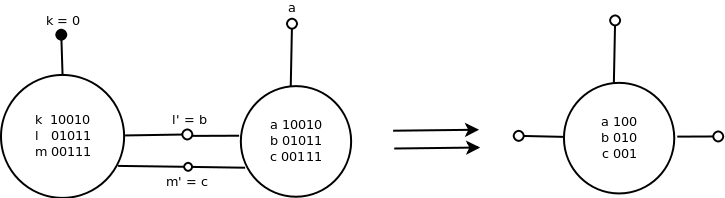
\includegraphics[width=0.01\textwidth]{3_2to3.png}
\caption{Получение константы}
\label{fig:constant}
\end{figure}
\end{proof}

\subsection{Получение отрицания}
\begin{lemma}
\label{eq:negate}
Пусть дан полный базис B. Тогда, применением операций $|_{x_1, x_2}$, подстановки констант,
и проекции к предикатам из B, можно получить предикат $\pi_{negate}$.
\end{lemma}

\begin{proof}
$\exists \pi \in B, \pi \notin K \Rightarrow \exists \alpha_1, \alpha_2 \in \Pi$,
$\alpha_1\&\alpha_2=\beta, \beta \notin \Pi$, причем эти наборы должны отличаться как минимум по двум переменным $x_i, x_{j}$.
Таким образом, подставив вместо всех общих переменных этих наборов соответствующие константы 0 и 1, применив операцию 
$\perp_{\forall x_t, t \neq i,j}$
(чтобы оставить в точности две необходимых для сохранения свойства $\pi \notin K$ переменных $x_i, x_j$), 
получим предикат-отрицание $\pi_{negate}$.
\begin{figure}[htb]
\centering
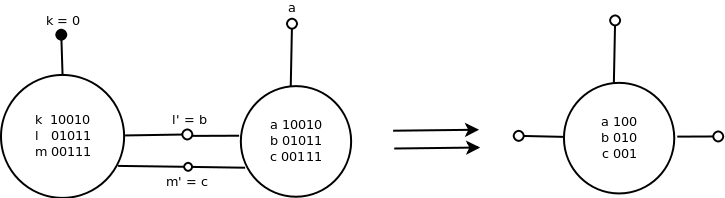
\includegraphics[width=0.01\textwidth]{3_2to3.png}
\caption{Получение $\pi_{neg}$}
\label{fig:negation}
\end{figure}

\end{proof}

\begin{corollary}
Обосновали добавление операции отрицания i-той переменной $\neg_i$ к множеству стандартных операций.
\end{corollary}

\clearpage
\section{Планарность}
\subsection{Планарные базисы}

\begin{figure}[htb]
\centering
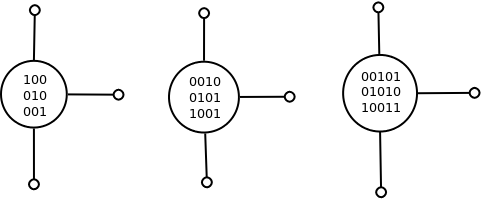
\includegraphics[width=0.5\textwidth]{scheff3.png}
\caption{Шефферовы предикаты от 3 переменных}
\label{fig:sheff}
\end{figure}

\label{planar_basis}
\begin{proposition}
Шефферовы базисы на рис. \ref{fig:sheff} являются планарными.
\end{proposition}
\begin{proof}
Пусть дана предикатная схема $\Sigma$, граф которой, при укладке на плоскость, содержит
реберные пересечения. Так как в базисе $B=\{\pi_{symm}^3\}$ можно планарной схемой реализовать предикат 
$\pi_{linear}, \Pi_{linear} = \{ (001), (010), (100), (111) \}$, то замещая каждое реберное пересечение в схеме на 
3 предиката ($\pi_{linear}$) по схеме \ref{fig:xor}, получаем планарную реализацию требуемого предиката
в базисе B.
\end{proof}

\textbf{Замечание.} При преобразовании непланарной схемы в базисе $B=\{\pi_{symm}^3\}$
по вышеописанному алгоритму, сложность схемы в смысле количества предикатов возрастает на $3*3*k=9*k$, где $k$~-- число реберных
пересечений графа предикатной схемы, $3$~-- число предикатов, необходимое для реализации $\pi_{linear}$.

\begin{figure}[htb]
\centering
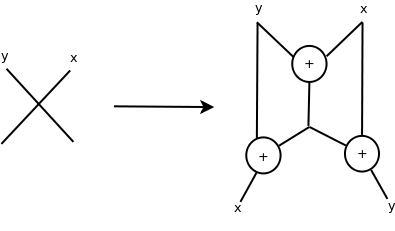
\includegraphics[width=0.5\textwidth]{intersection.png}
\caption{Получение планарной схемы}
\label{fig:xor}
\end{figure}



%\textbf{Лемма.} Система из $\{\pi_1 \notin SM, \pi_{neq}, \Pi_neq = \{ (01), (10) \}\}$ полна.
%\textbf{Доказательство.} 

\begin{lemma}
\label{eq:lemma_sm}
Если $\pi \notin SM$, то, применяя операции $\perp_i$ и $\neg_i$,
можно получить $\pi_{min} \notin SM$, причем $\pi_{min}$ будет являться расширением симметричного предиката.
\end{lemma}

\begin{proof}
Рассмотрим $\pi_{min} \notin SM$ такой, что $\forall i, \pi_1 = \pi_{min} \perp_{x_i}$,
$\pi_1 \in SM$.
Пусть $\beta = (\beta_1, \dots, \beta_k)$~-- набор, $\notin \pi_{min}$, полученный в результате применения какой-то несамодвойственной функции.
Заметим, что $\beta \neq \forall \alpha \in \pi$. Однако, для соблюдения верхнего условия,
$\Pi_{min}$ должно содержать наборы 
$(\bar{\beta_1}, \beta_2, \dots, \beta_k), (\beta_1, \bar{\beta_2}, \dots, \beta_k), \dots, (\beta_1, \beta_2, \dots, \bar{\beta_k})$.

Нетрудно видеть, что набор $(\bar{\beta_1}, \bar{\beta_2}, \dots, \bar{\beta_k})$~-- существенный для $\pi_{min}$.

Так как класс $SM$ замкнут относительно $\neg_i$, применяя эту операцию к $\pi_{min}$ можно получить $\pi_{min}^1$,
такой что набор $(\sigma, \sigma, \dots, \sigma)$ является для него существенным, а сам $pi_{min}^1$ является расширением 
симметричного предиката.
\end{proof}

\begin{corollary}
$\pi \notin SM \Longrightarrow \exists \pi_{min} \notin SM, 
\alpha = (\sigma, \sigma, \dots, \sigma) \notin \Pi_{min}, \sigma \in \{0, 1\}$.
\end{corollary}

\begin{lemma}
\label{eq:super_new}
Пуcть $\pi \notin SM$, $\pi$~-- расширение симметричного предиката $\pi_{symm}^3$. 
Тогда, применяя операции планарной суперпозиции, можно получить планарную реализацию $\pi_{linear}$.
\end{lemma}

\begin{proof}
По условию, $\Pi = Pi_{symm}^3 \bigcup A$, где
$ A \subseteq(\alpha \bar{\alpha} \alpha), (\alpha \alpha \bar{\alpha}), (\alpha \bar{\alpha} \alpha), (\alpha \alpha \alpha) \} $.

Заметим, что во всех наборах из A от 2 до 3 координат равны $\alpha$, и $|A| = k, 1 \leq k \leq 4$.
Таким образом, применением операцию суперпозиции с отождествлением по 2 переменным предиката $\pi(x_1, x_2, x_3)$ 
и предиката $\pi_1(y_1, y_2)$, $\Pi_1 = \{ (\bar{\alpha}, \bar{\alpha}), (\bar{\alpha}, \alpha), (\alpha, \bar{\alpha})\}$,
$(\pi|\pi_1)_{x_{i_1}=y_1, x_{i_2} =y_2}$, 

где $i_1 \neq i_2 \neq j$,
\[ j = \left \{
  \begin{array}{l l}
     t & \quad \text{если $\exists \widetilde{\beta}=(\beta_1, \beta_2, \beta_3) \in A, \beta_t=\bar{\alpha}$ }\\
     \forall t \in [1, 3] & \quad \text{если $A = \{ (\alpha, \alpha, \alpha)\}$}
            \end{array} \right. \]

Остается получить предикат $\pi_1$.
Рассмотрим 2 случая. 

1. Пусть $A \neq (\alpha, \alpha, \alpha)$. Тогда
$\exists! \widetilde{\beta}=(\beta_1, \beta_2, \beta_3) \in A, \beta_t=\bar{\alpha}$. Подставив на место $t$-ой переменной
предиката $\pi$ константу $\bar{\alpha}$, и спроецировав по переменной t получим: 
$(\pi(x_1, x_2, x_3)|_{x_t=\bar{\alpha}} \perp_{x_t} )$ = 
$\pi_1'(x_1, x_2), \Pi_1'=\{(\bar{\alpha}, \alpha), (\alpha, \bar{\alpha}), (\alpha, \alpha)\}$, из которого искомый предикат
$\pi_1$ получается применением операции $\neg$.

В базисе из симметричного предиката 

$\pi_{linear}(z_1, y_2, x_3)=(((\pi(x_1, x_2, x_3)|\pi(y_1, y_2, y_3))_{x_1=y_1}|\pi(z_1, z_2, z_3) )_{y_3=z_3, x_2=z_1}) \perp_{z_2, y_3, x_2}$


2. Пусть $A = (\alpha, \alpha, \alpha)$. Тогда $\pi=\pi_{linear}$. Лемма доказана. 
\end{proof}

\begin{lemma}
Если $\pi(x_1, \dots, x_n) = \pi_{symm}^n, n > 3$, то, 
применяя операции подстановки констант и $\perp$, можно получить $\pi_{symm}^{n-1}$.
\end{lemma}

\begin{proof}
Так как 
$\pi \notin SM, \exists \widetilde{\alpha} = (\alpha, \dots, \alpha)$, $\pi$ не сохраняет $\widetilde{\alpha}$.
Тогда 
$\pi_1 = ( (\pi|_{x_1=\alpha}) \perp_{x_1} )$, где $\pi_1(x_1, \dots, x_{n-1}) = \pi_{symm}^{n-1}$
\end{proof}

\begin{lemma}
\label{eq:svedenie}
Если $\pi(x_1, \dots, x_n) \notin SM, n > 3$, то, применяя операции подстановки констант, $\neg$ и $\perp$,
можно получить $\pi_1(x_1, \dots, x_{n-1}) \notin SM$.
\end{lemma}

\begin{proof}
По следствию из \ref{eq:lemma_sm}, 
$\exists \pi_{min} \notin SM, \alpha=(\sigma, \dots, \sigma) \notin \Pi_{min}$. Тогда предикат $\pi_1$, такой что
$\pi_1 = ( (\pi_{min}|_{x_1=\sigma}) \perp_{x_1} )$, не принадлежит $SM$, и зависит от $n-1$ переменной.
\end{proof}
%\label{eq:3tuples}
%\textbf{Следствие.} Пусть $\pi(x_1, x_2, x_3) \notin SM$. 
%Тогда : $\pi_1 = (((\pi SELECT x_1=\bar{\alpha}) PROJECT x_1)$ и 
%$\Pi_1 = \{ (\bar{\alpha}\alpha), (\alpha\bar{\alpha}), (\alpha\alpha) \}$

\subsection{Алгоритм планарного сведения}

\begin{theorem}
Пусть дана непланарная предикатная схема $\Sigma$ в полном предикатном базисе $B$, все элементы которого зависят 
не более чем от 3 переменных. Тогда из $\Sigma$, применением операций планарной суперпозиции, можно получить схему $\Sigma'$,
реализующую тот же предикат, что и $\Sigma$, но являющуюсь планарной.
\end{theorem}
\begin{proof}
Приведем конструктивный алгоритм преобразования исходной схемы.

Так как $B$~-- полный базис, то по леммам \ref{eq:const} и \ref{eq:negate} получаем константы и $\pi_{negate}$. 
Таким образом, становится доступным весь набор операций планарной суперпозиции. 

По лемме \ref{eq:lemma_sm} получаем предикат $\pi_{min} \notin SM$, где $\pi_{min}$~-- либо симметричный предикат, 
либо его расширение\footnote{Естественно, не изменяющее существенность}. 

В случае, если $\pi_{min}$ не является симметричным предикатом, применением операций планарной суперпозиции к $\pi_{min}$,
 получаем планарную реализацию $\pi_{linear}$ по лемме \ref{eq:super_new}.

Заменив каждое реберное пересечение на 3 предиката $\pi_{linear}$, получаем планарную схему.
\end{proof}

\begin{corollary}
Пусть дана непланарная предикатная схема $\Sigma$ в полном предикатном базисе $B$.
Тогда из $\Sigma$, применением операций планарной суперпозиции, можно получить схему $\Sigma'$,
реализующую тот же предикат, что и $\Sigma$, но являющуюсь планарной.
\end{corollary}

\begin{proof}
По лемме \ref{eq:svedenie}, из $\pi \in B, \pi \notin SM$, применением операций планарной
суперпозиции, можно получить $\pi_1(x_1, x_2, x_3) \notin SM$, и дальше воспользоваться результатом теоремы.
\end{proof}

\clearpage
\subsection{Примеры планарных сведений некоторых предикатов}

\begin{figure}[htb]
\centering
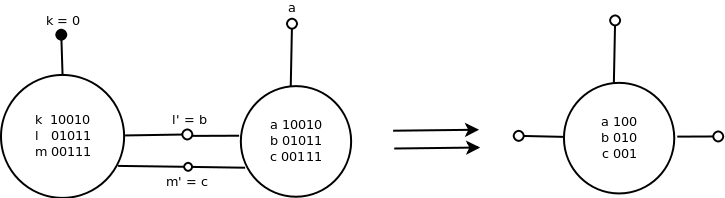
\includegraphics[width=1.0\textwidth]{3_2to3.png}
\caption{Сведение $\pi_5^3$ к $\pi_{symm}^3$ }
\label{fig:3_2to3}
\end{figure}

\ref{eq:svedenie}, как показано на рисунке \ref{fig:4to3}
\begin{figure}[htb]
 \centering
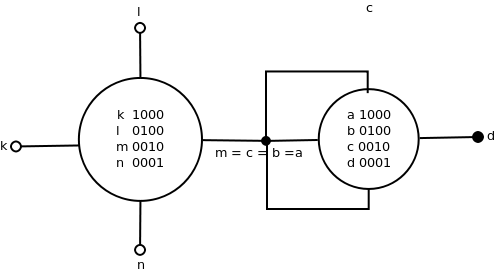
\includegraphics[width=0.6\textwidth]{4to3.png}
\caption{Сведение $\pi_{symm}^4$ к $\pi_{symm}^3$ }
\label{fig:4to3}
\end{figure}

%\begin{figure}[htb]
%\centering
%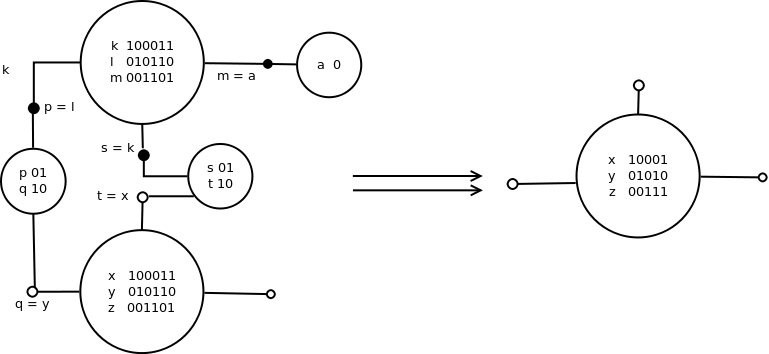
\includegraphics[width=1.0\textwidth]{3_3to3_2.png}
%\caption{Сведение $\pi_{symm+3}^3$ к $\pi_{symm+2}^3$}
%\label{fig:3_3to3_2}
%\end{figure}

%\begin{figure}[htb]
%\centering
%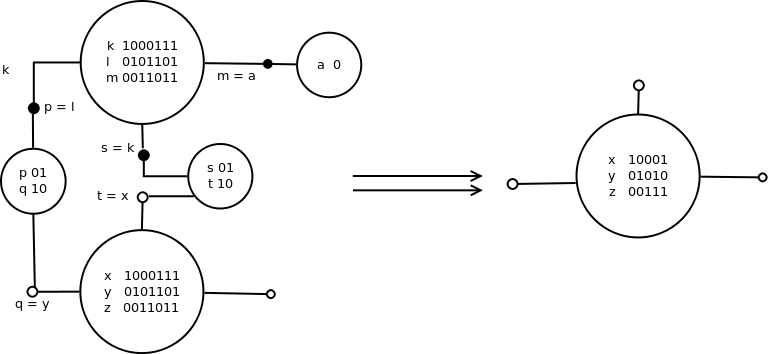
\includegraphics[width=1.0\textwidth]{3_4to3_2.png}
%\caption{Сведение $\pi_{symm+4}^3$ к $\pi_{symm+2}$}
%\label{fig:3_4to3_2}
%\end{figure}

\clearpage
\section{Получение минимальных схем в базисе $\pi_{symm}^3$}
В Теореме 1 было показан алгоритм планарного сведения произвольного полного базиса к $\pi_{symm}^3$. 
В этой главе будут рассмотрены вопрос синтеза планарных предикатных схем по заданной функции и 
приведены примеры минимальных планарных схем для некоторых функций.


\begin{figure}[htb]
\centering
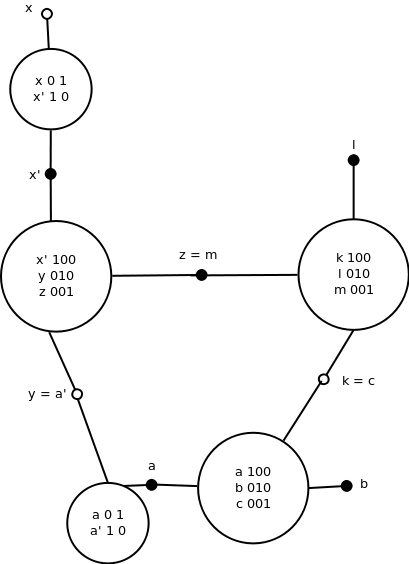
\includegraphics[width=0.7\textwidth]{min_and.png}
\caption{Схема для $\pi_{and}$}
\label{fig:and}
\end{figure}

% Список цитируемой литературы
\clearpage
\addcontentsline{toc}{section}{Список цитируемой литературы}
\thebibliography{99}
\RBibitem{Shu09}
    \by М.~С.~Шуплецов
    \paper Оценки высокой степени точности для сложности предикатных схем в~некоторых базисах
    \inbook Физико-математические науки
    \serial Уч\"eн. зап. Казан. гос. ун-та. Сер. Физ.-матем. науки
    \yr 2009
    \vol 151
    \issue 2
    \pages 173--184
    \publ Изд-во Казанского ун-та
    \publaddr Казань
    \mathnet{http://mi.mathnet.ru/uzku760}

\bibitem{Shu11}Методы синтеза и оценки сложности схем, построенных из элементов предикатного типа, диссертация

\bibitem{CSP10} Handbook of Constraint Programming, ISBN 9780444527264; 2010 г.

\bibitem{Shaeffer78} Schaefer, Thomas J. (1978). 
``The Complexity of Satisfiability Problems''. STOC 1978. pp. 216–226. doi:10.1145/800133.804350.

\bibitem{Zarank54} Zarankiewicz, K. "On a Problem of P. Turán Concerning Graphs." Fund. Math. 41, 137-145, 1954. 

\bibitem{Prosc89} Arnborg, S.; Proskurowski, A. (1989), 
``Linear time algorithms for NP-hard problems restricted to partial k-trees'',
Discrete Applied Mathematics 23 (1): 11–24, doi:10.1016/0166-218X(89)90031-0.

\bibitem{Gott10} 
Georg Gottlob, Reinhard Pichler, and Fang Wei. 2010. Bounded treewidth as a key to tractability of knowledge representation and reasoning. Artif. Intell. 174, 1 (January 2010), 105-132. DOI=10.1016/j.artint.2009.10.003 http://dx.doi.org/10.1016/j.artint.2009.10.003

\bibitem{Diestel00}
Diestel, Reinhard (2000), Graph Theory, Graduate Texts in Mathematics, 
173, Springer-Verlag, ISBN 0-387-98976-5.

\bibitem{Boedlander96}
H. L. Bodlaender, A linear-time algorithm for finding 
tree-decompositions of small
treewidth, SIAM J. Comput. 25 (1996), 1305–1317

\bibitem{Marchenkov}
C.C. Марченков, ``Предполнота замкнутых классов в $P_k$: предикатный подход'', Проблемы Кибернетики

\bibitem{Zhuk}
Жук, монография

\endthebibliography

\end{document}
